	\section{Wykresy}

\begin{figure}[h!]
	\centering
	\begin{subfigure}[b]{0.3\linewidth}
		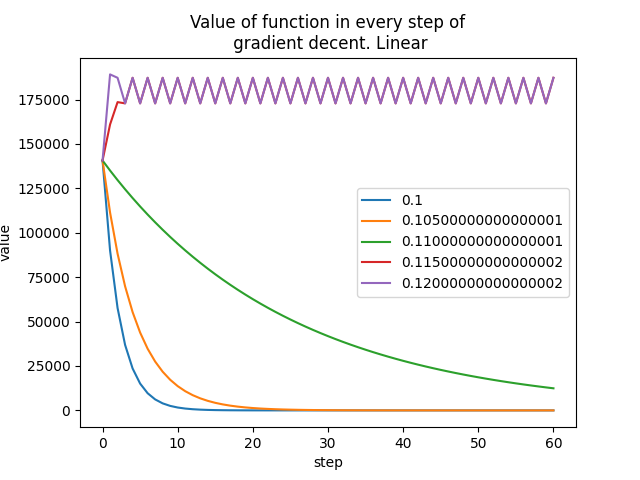
\includegraphics[width=\linewidth]{photos/booth_vals_lin.png}
		\caption{Skala liniowa}
	\end{subfigure}
	\begin{subfigure}[b]{0.3\linewidth}
		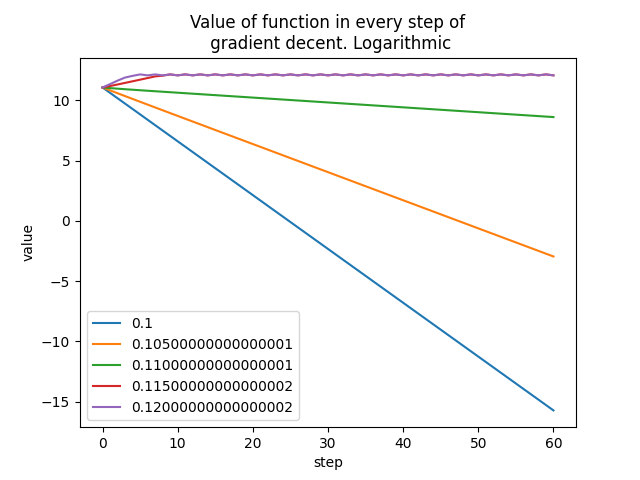
\includegraphics[width=\linewidth]{photos/booth_vals_log.png}
		\caption{Skala logarytmiczna}
	\end{subfigure}
	\caption{Charakterystyka wartości funkcji booth od kroku w zależności od wartości $\beta$.}
	\begin{subfigure}[b]{0.3\linewidth}
		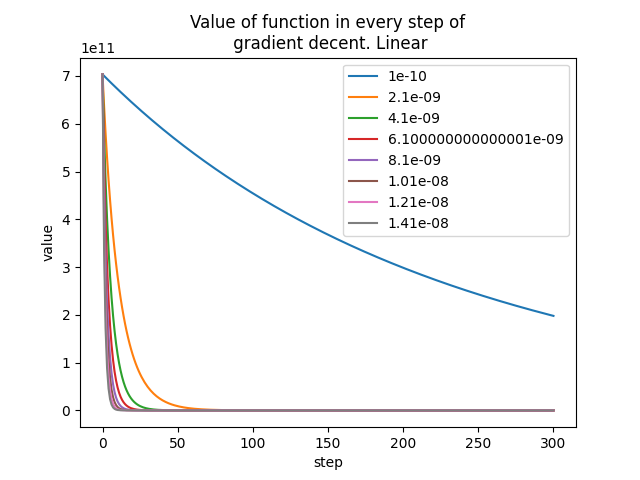
\includegraphics[width=\linewidth]{photos/f1_vals_lin.png}
		\caption{Skala liniowa}
	\end{subfigure}
	\begin{subfigure}[b]{0.3\linewidth}
		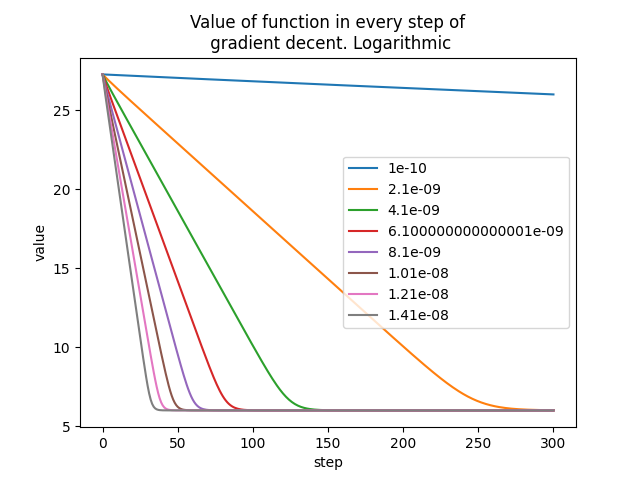
\includegraphics[width=\linewidth]{photos/f1_vals_log.png}
		\caption{Skala logarytmiczna}
	\end{subfigure}
	\caption{Charakterystyka wartości funkcji CEC2017 f1 od kroku w zależności od wartości $\beta$.}
	\begin{subfigure}[b]{0.3\linewidth}
		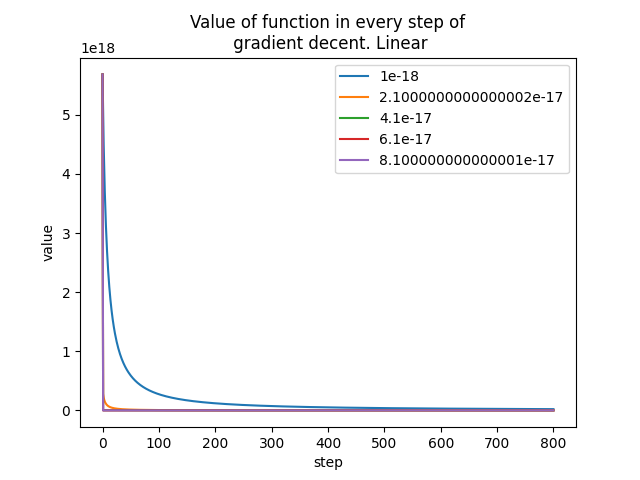
\includegraphics[width=\linewidth]{photos/f2_vals_lin.png}
		\caption{Skala liniowa}
	\end{subfigure}
	\begin{subfigure}[b]{0.3\linewidth}
		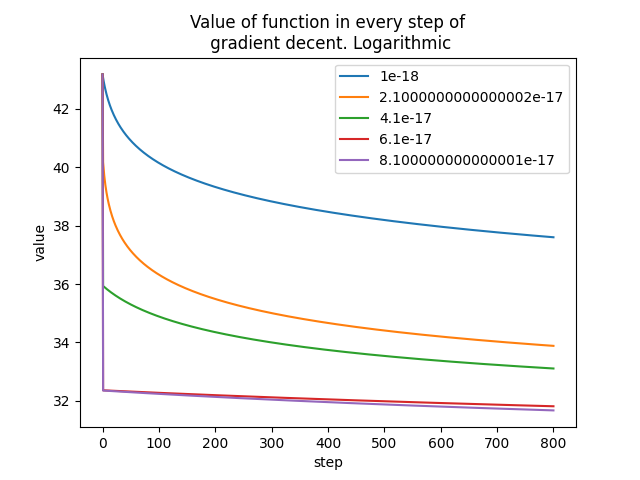
\includegraphics[width=\linewidth]{photos/f2_vals_log.png}
		\caption{Skala logarytmiczna}
	\end{subfigure}
	\caption{Charakterystyka wartości funkcji CEC2017 f2 od kroku w zależności od wartości $\beta$.}
	\begin{subfigure}[b]{0.3\linewidth}
		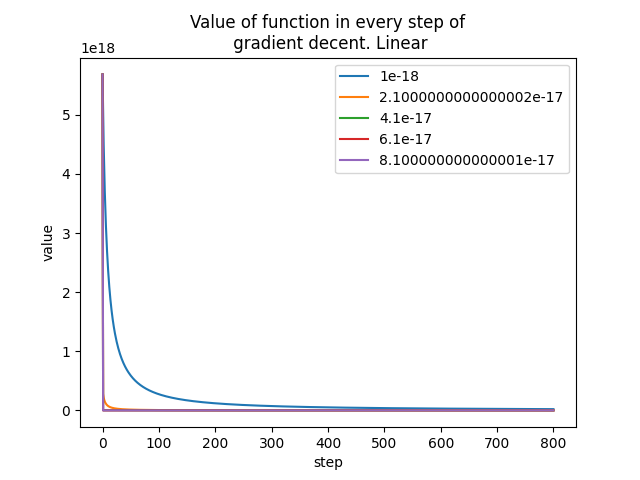
\includegraphics[width=\linewidth]{photos/f2_vals_lin.png}
		\caption{Skala liniowa}
	\end{subfigure}
	\begin{subfigure}[b]{0.3\linewidth}
		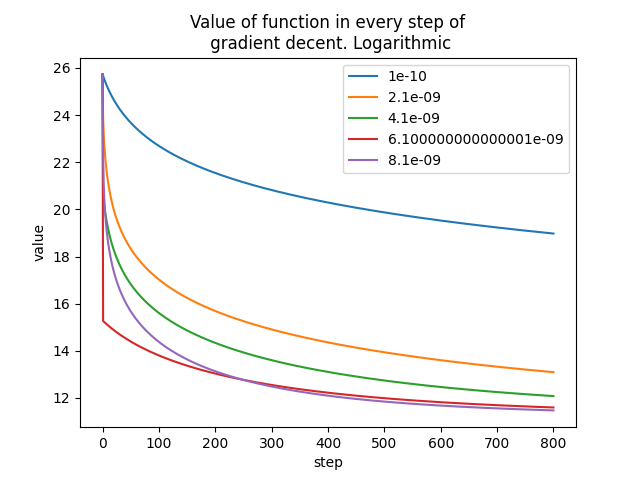
\includegraphics[width=\linewidth]{photos/f3_vals_log.png}
		\caption{Skala logarytmiczna}
	\end{subfigure}
	\caption{Charakterystyka wartości funkcji CEC2017 f3 od kroku w zależności od wartości $\beta$.}
\end{figure}


	\begin{figure}[h!]
		\centering
		\begin{subfigure}[b]{0.45\linewidth}
			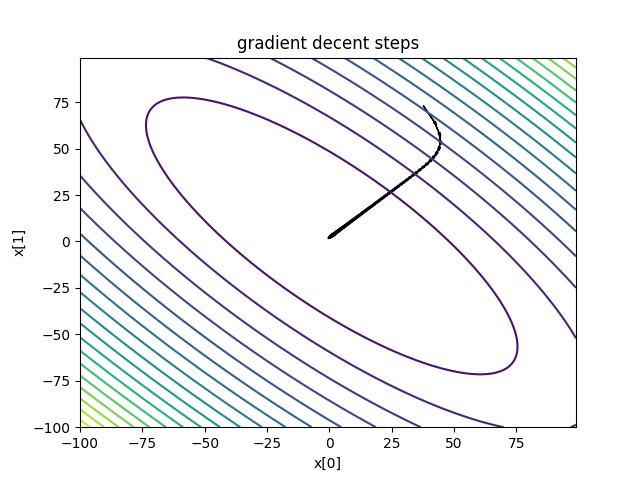
\includegraphics[width=\linewidth]{photos/booth1.png}
		\end{subfigure}
		\begin{subfigure}[b]{0.45\linewidth}
			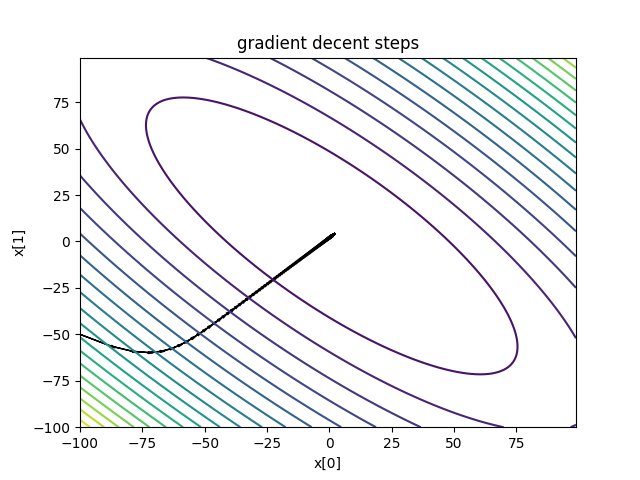
\includegraphics[width=\linewidth]{photos/booth2.png}
		\end{subfigure}
		\begin{subfigure}[b]{0.45\linewidth}
			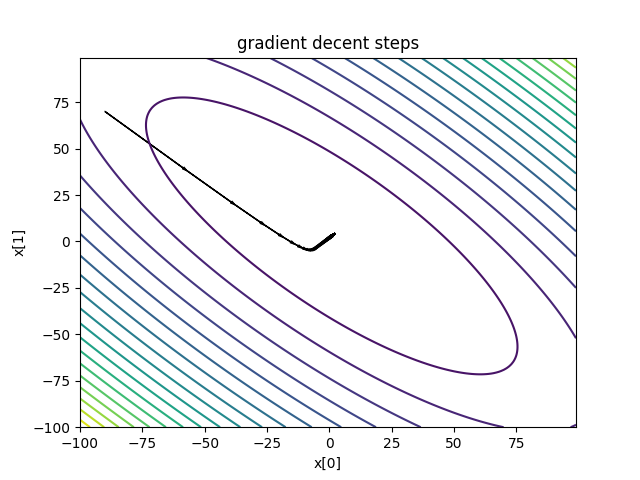
\includegraphics[width=\linewidth]{photos/booth3.png}
		\end{subfigure}
			\caption{Zbieżność funkcji booth. $\beta = 0.11$.}
	\end{figure}
	\newpage
	
	\begin{figure}[h!]
	\centering
	\begin{subfigure}[b]{0.45\linewidth}
		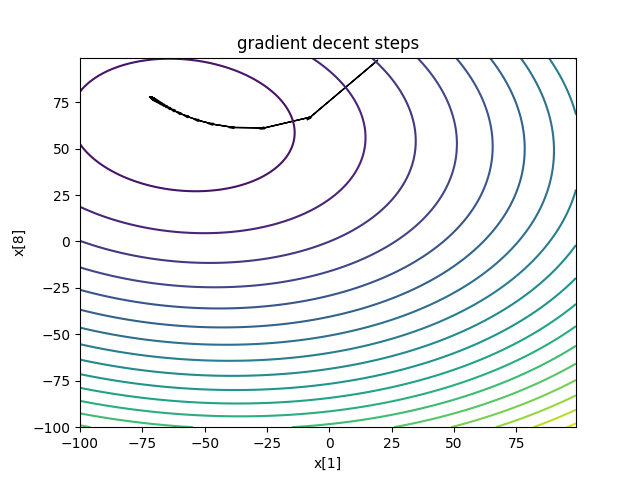
\includegraphics[width=\linewidth]{photos/f1_1_0.png}
		\end{subfigure}
		\begin{subfigure}[b]{0.45\linewidth}
			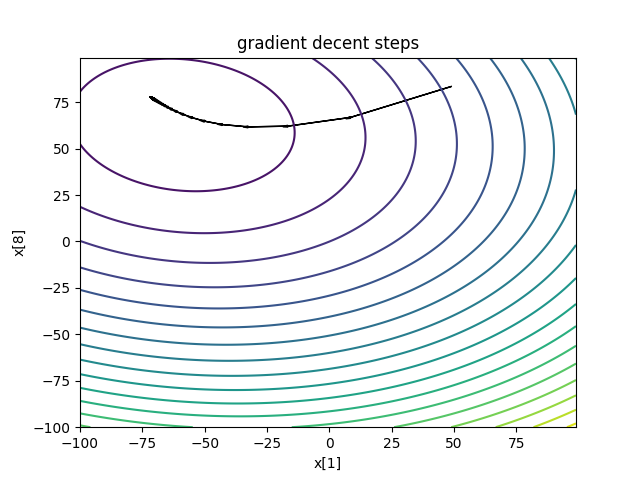
\includegraphics[width=\linewidth]{photos/f1_2_0.png}
		\end{subfigure}
		\begin{subfigure}[b]{0.45\linewidth}
			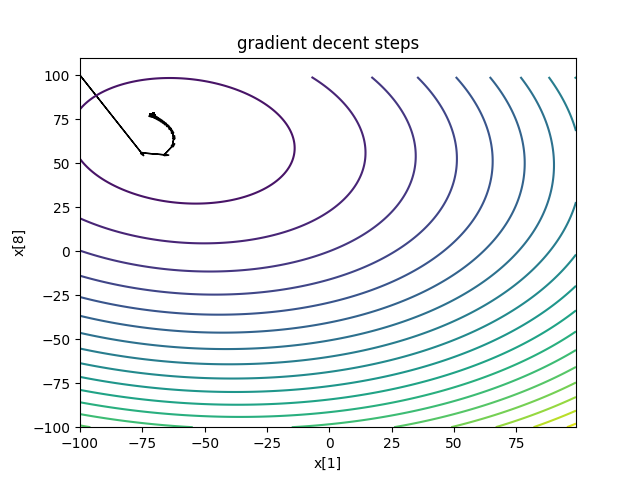
\includegraphics[width=\linewidth]{photos/f1_3_0.png}
		\end{subfigure}
		\caption{Zbieżność CEC2017 f1. Wymiary 1 i 8.}
	\end{figure}
	\newpage
	\begin{figure}[h!]
		\centering
		\begin{subfigure}[b]{0.45\linewidth}
			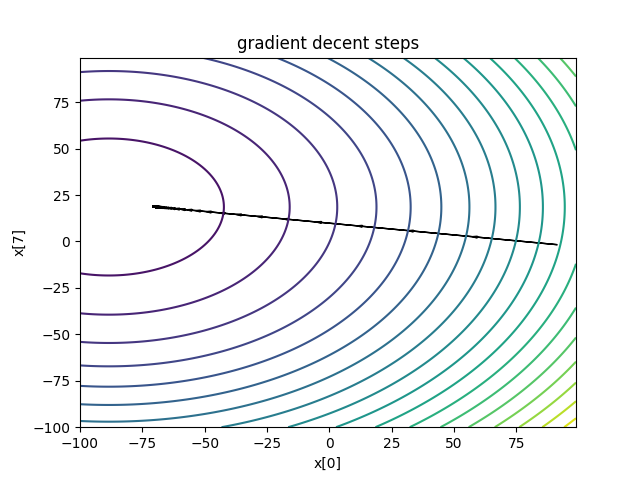
\includegraphics[width=\linewidth]{photos/f1_1_1.png}
		\end{subfigure}
		\begin{subfigure}[b]{0.45\linewidth}
			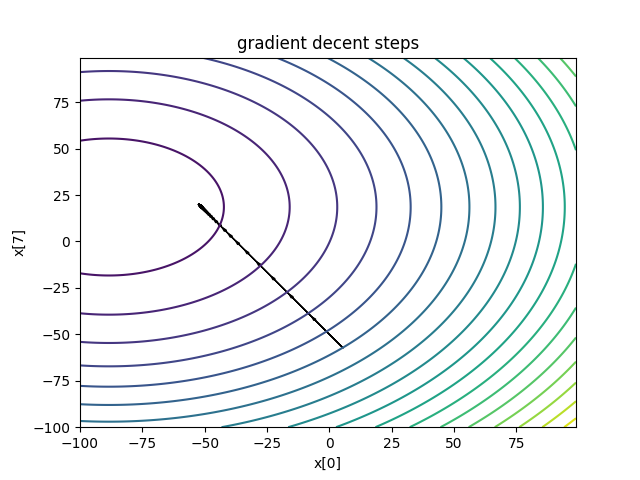
\includegraphics[width=\linewidth]{photos/f1_2_1.png}
		\end{subfigure}
		\begin{subfigure}[b]{0.45\linewidth}
			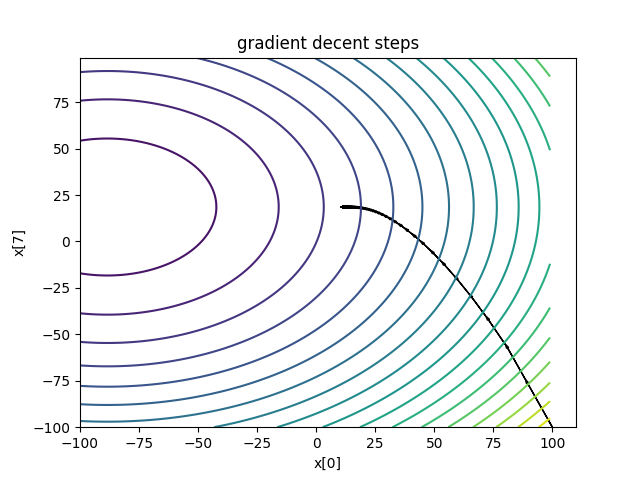
\includegraphics[width=\linewidth]{photos/f1_3_1.png}
		\end{subfigure}
		\caption{Zbieżność CEC2017 f1. Wymiary 0 i 7.}
	\end{figure}
	\newpage
	\begin{figure}[h!]
		\centering
		\begin{subfigure}[b]{0.45\linewidth}
			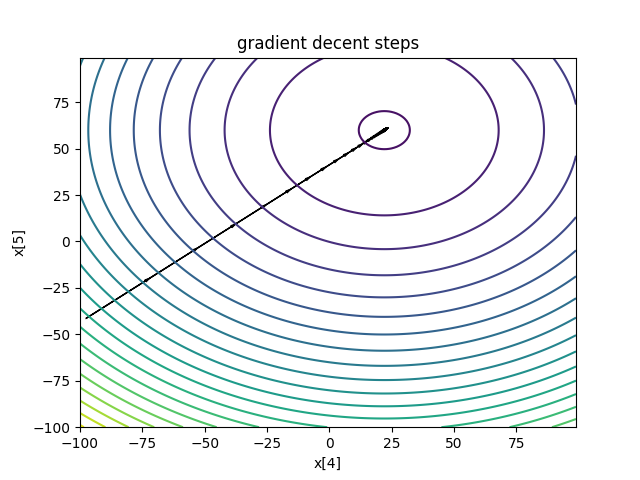
\includegraphics[width=\linewidth]{photos/f1_1_2.png}
		\end{subfigure}
		\begin{subfigure}[b]{0.45\linewidth}
			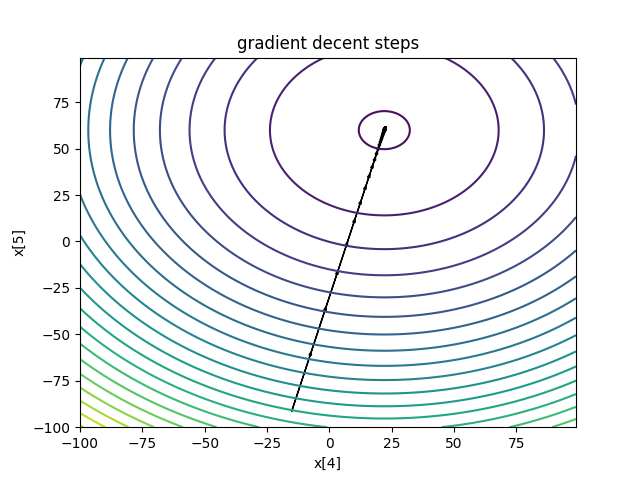
\includegraphics[width=\linewidth]{photos/f1_2_2.png}
		\end{subfigure}
		\begin{subfigure}[b]{0.45\linewidth}
			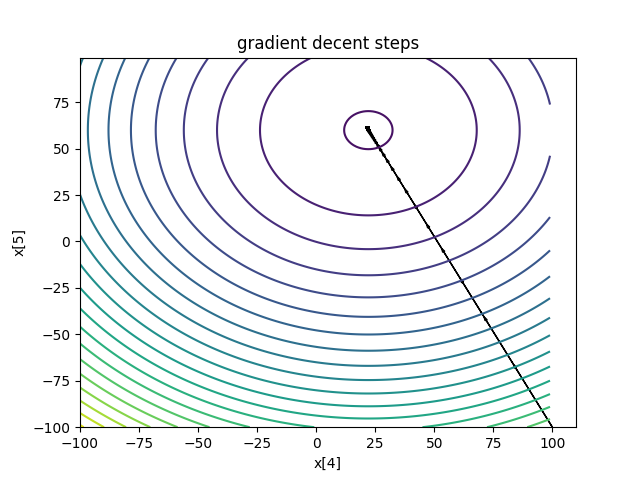
\includegraphics[width=\linewidth]{photos/f1_3_2.png}
		\end{subfigure}
		\caption{Zbieżność CEC2017 f1. Wymiary 4 i 5.}
	\end{figure}
	\newpage
	
	\begin{figure}[h!]
		\centering
		\begin{subfigure}[b]{0.45\linewidth}
			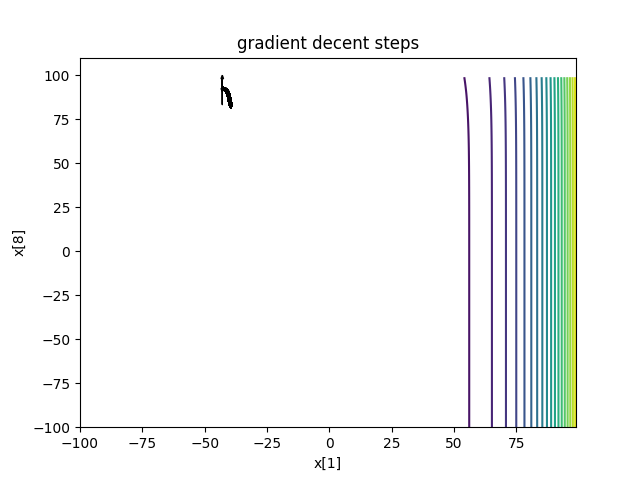
\includegraphics[width=\linewidth]{photos/f2_1_0.png}
		\end{subfigure}
		\begin{subfigure}[b]{0.45\linewidth}
			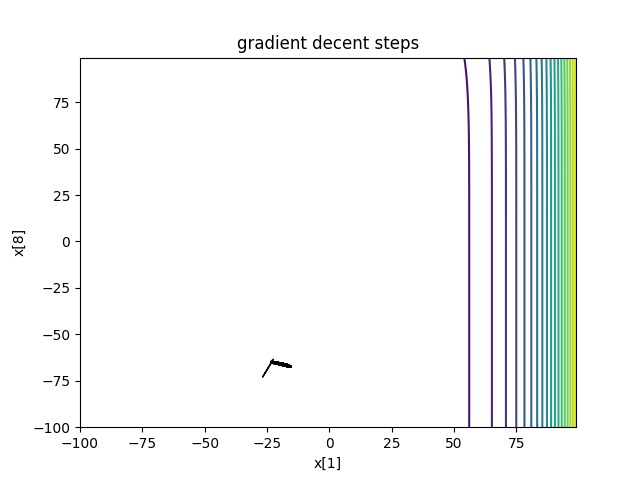
\includegraphics[width=\linewidth]{photos/f2_2_0.png}
		\end{subfigure}
		\begin{subfigure}[b]{0.45\linewidth}
			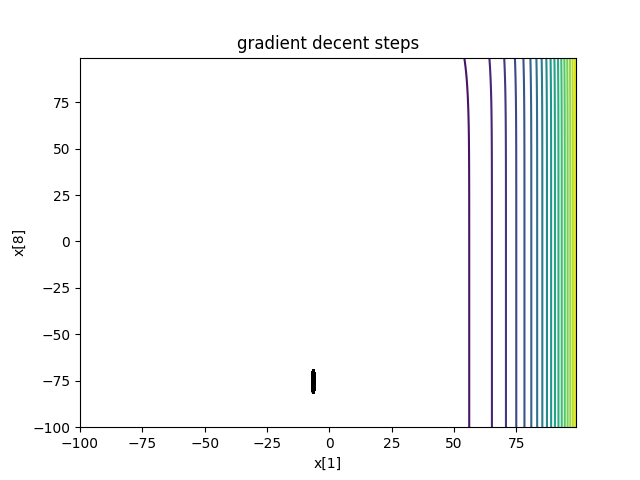
\includegraphics[width=\linewidth]{photos/f2_3_0.png}
		\end{subfigure}
		\caption{Zbieżność CEC2017 f2. Wymiary 1 i 8.}
	\end{figure}
	\newpage
	\begin{figure}[h!]
		\centering
		\begin{subfigure}[b]{0.45\linewidth}
			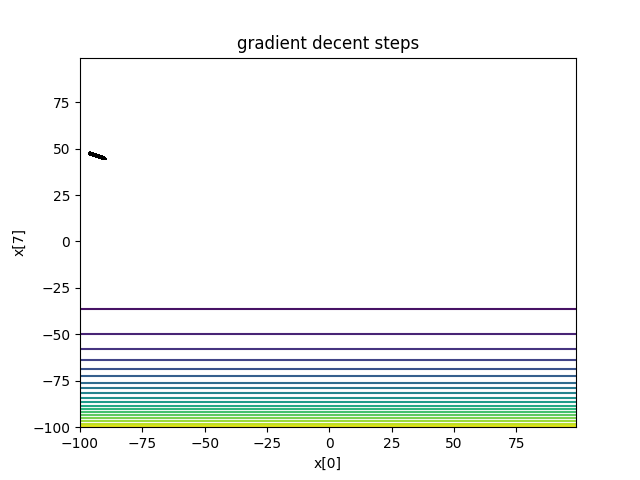
\includegraphics[width=\linewidth]{photos/f2_1_1.png}
		\end{subfigure}
		\begin{subfigure}[b]{0.45\linewidth}
			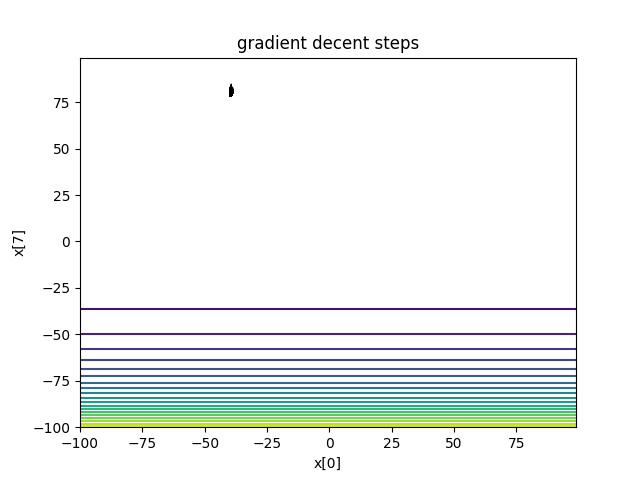
\includegraphics[width=\linewidth]{photos/f2_2_1.png}
		\end{subfigure}
		\begin{subfigure}[b]{0.45\linewidth}
			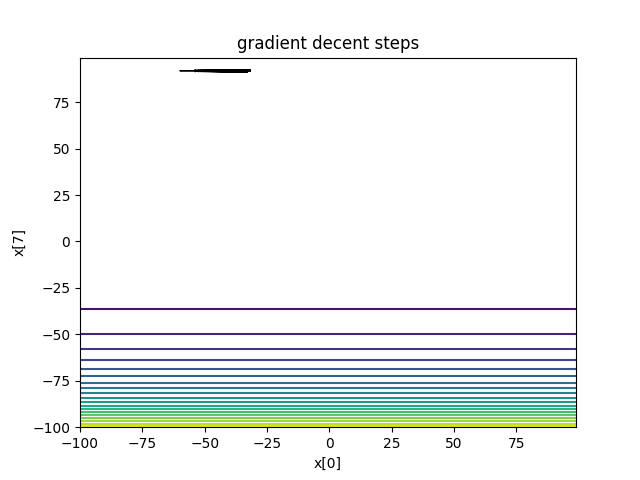
\includegraphics[width=\linewidth]{photos/f2_3_1.png}
		\end{subfigure}
		\caption{Zbieżność CEC2017 f2. Wymiary 0 i 7.}
	\end{figure}
	\newpage
		\begin{figure}[h!]
		\centering
		\begin{subfigure}[b]{0.45\linewidth}
			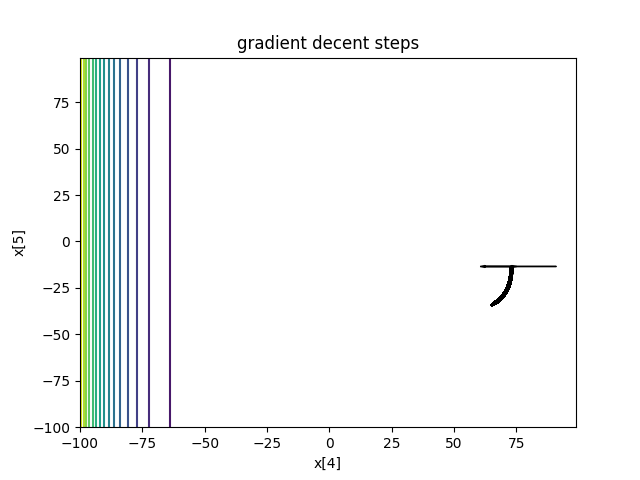
\includegraphics[width=\linewidth]{photos/f2_1_2.png}
		\end{subfigure}
		\begin{subfigure}[b]{0.45\linewidth}
			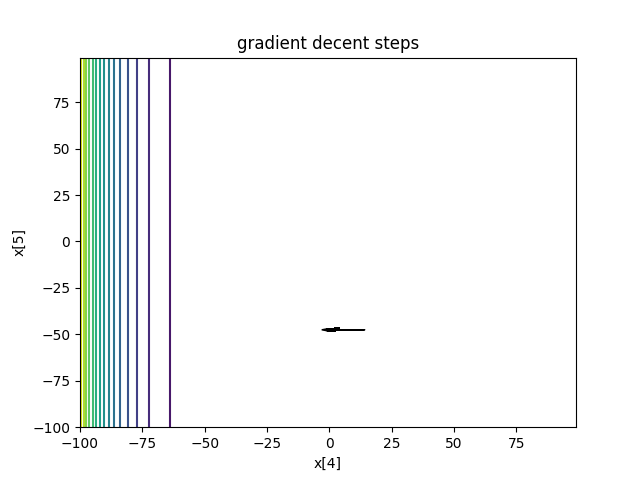
\includegraphics[width=\linewidth]{photos/f2_2_2.png}
		\end{subfigure}
		\begin{subfigure}[b]{0.45\linewidth}
			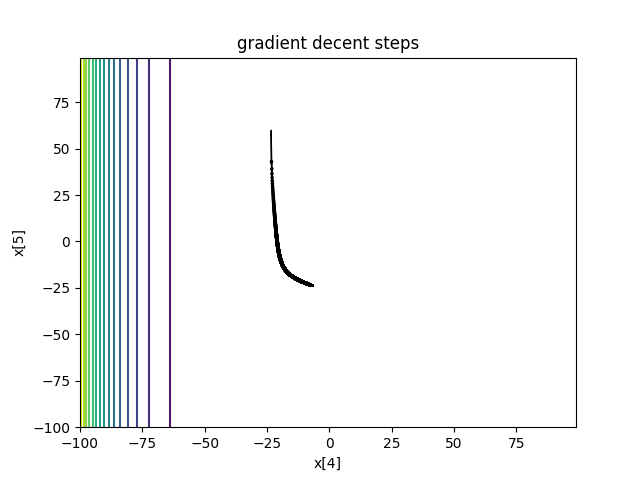
\includegraphics[width=\linewidth]{photos/f2_3_2.png}
		\end{subfigure}
		\caption{Zbieżność CEC2017 f2. Wymiary 4 i 5.}
	\end{figure}
	\newpage
	
	\begin{figure}[h!]
		\centering
		\begin{subfigure}[b]{0.45\linewidth}
			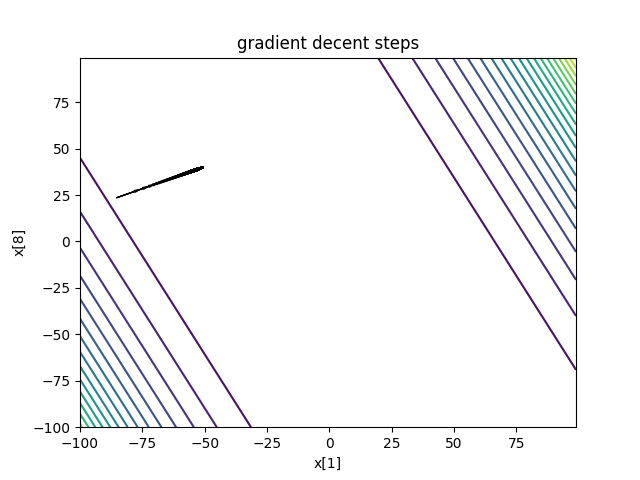
\includegraphics[width=\linewidth]{photos/f3_1_0.png}
		\end{subfigure}
		\begin{subfigure}[b]{0.45\linewidth}
			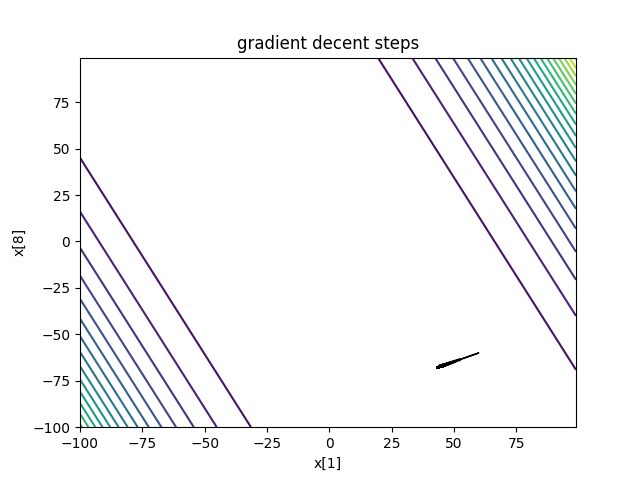
\includegraphics[width=\linewidth]{photos/f3_2_0.png}
		\end{subfigure}
		\begin{subfigure}[b]{0.45\linewidth}
			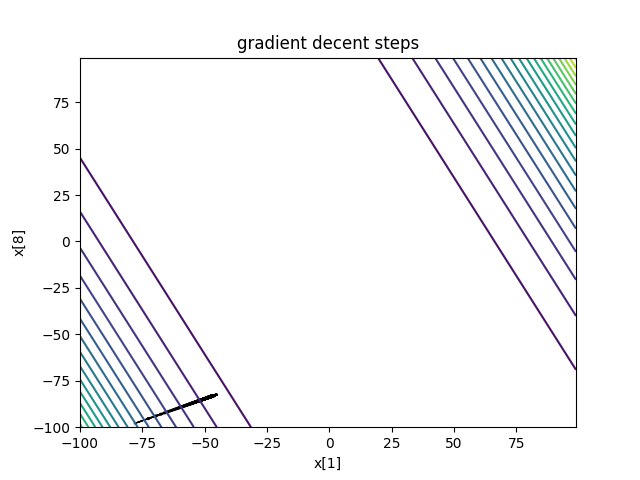
\includegraphics[width=\linewidth]{photos/f3_3_0.png}
		\end{subfigure}
		\caption{Zbieżność CEC2017 f3. Wymiary 1 i 8.}
	\end{figure}
	\newpage
	\begin{figure}[h!]
		\centering
		\begin{subfigure}[b]{0.45\linewidth}
			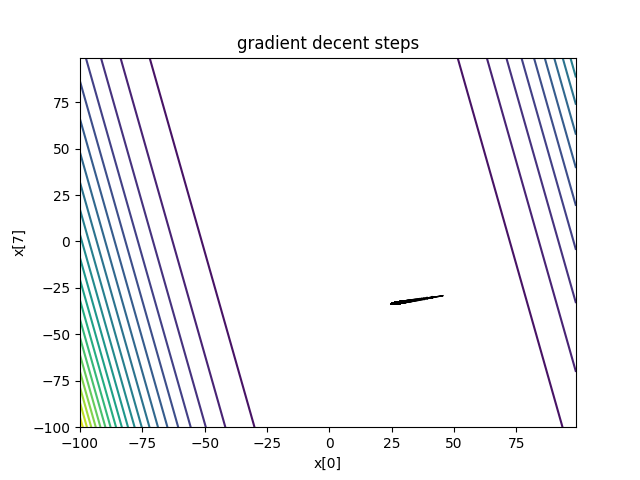
\includegraphics[width=\linewidth]{photos/f3_1_1.png}
		\end{subfigure}
		\begin{subfigure}[b]{0.45\linewidth}
			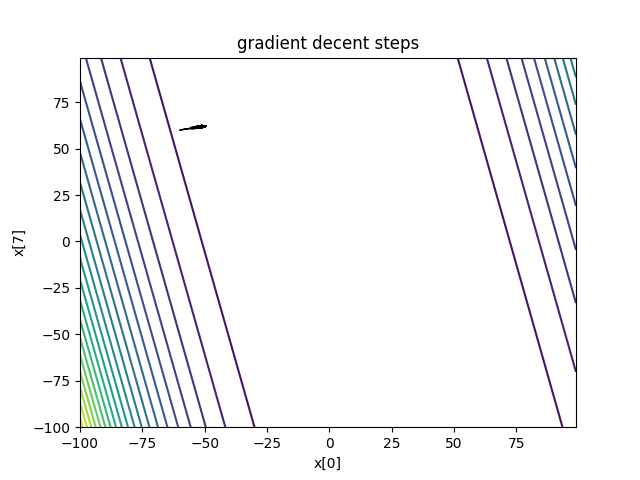
\includegraphics[width=\linewidth]{photos/f3_2_1.png}
		\end{subfigure}
		\begin{subfigure}[b]{0.45\linewidth}
			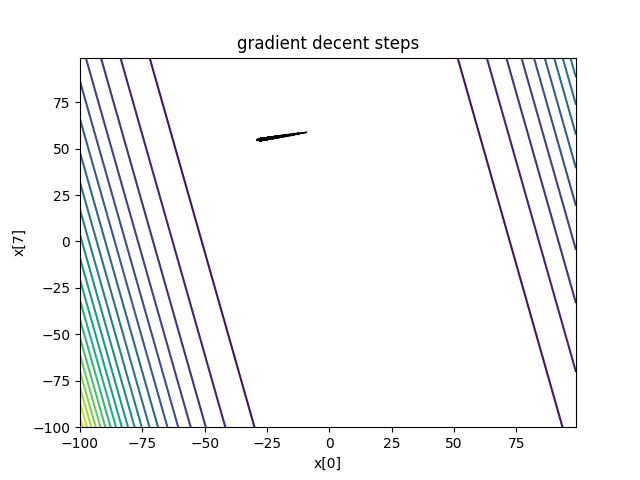
\includegraphics[width=\linewidth]{photos/f3_3_1.png}
		\end{subfigure}
		\caption{Zbieżność CEC2017 f3. Wymiary 0 i 7.}
	\end{figure}
	\newpage
	\begin{figure}[h!]
		\centering
		\begin{subfigure}[b]{0.45\linewidth}
			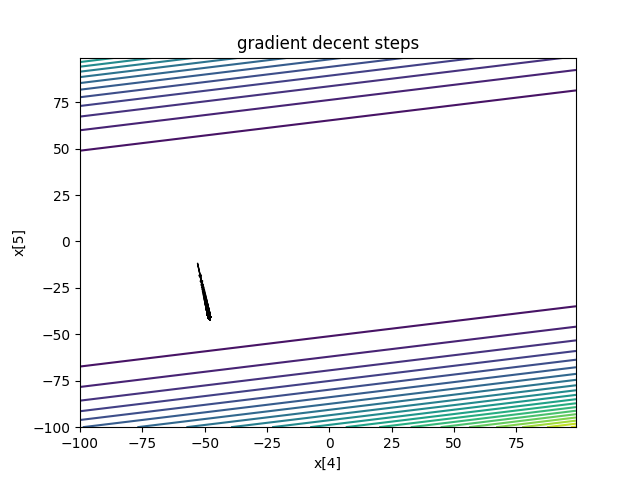
\includegraphics[width=\linewidth]{photos/f3_1_2.png}
		\end{subfigure}
		\begin{subfigure}[b]{0.45\linewidth}
			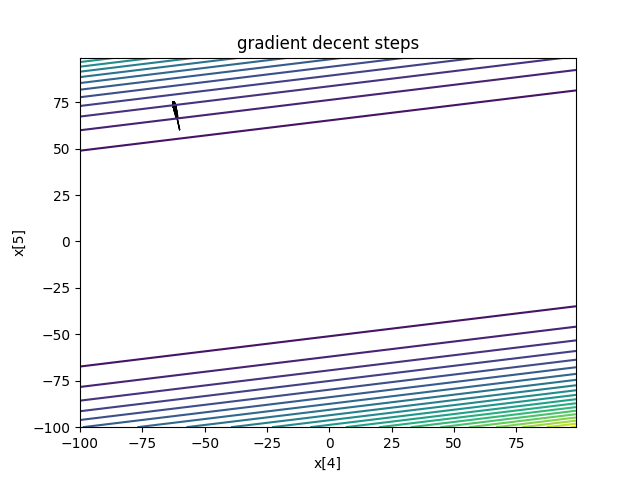
\includegraphics[width=\linewidth]{photos/f3_2_2.png}
		\end{subfigure}
		\begin{subfigure}[b]{0.45\linewidth}
			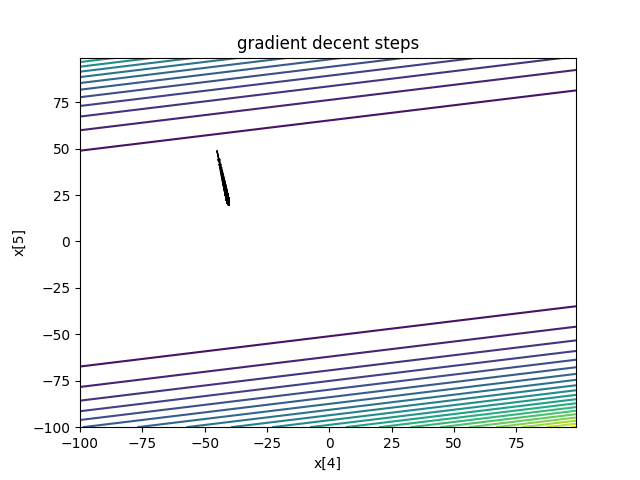
\includegraphics[width=\linewidth]{photos/f3_3_2.png}
		\end{subfigure}
		\caption{Zbieżność CEC2017 f3. Wymiary 4 i 5.}
	\end{figure}

